\documentclass{article}
\usepackage[utf8]{inputenc}

\title{Generating Sentences with DANN and Editing Prototypes}
\author{Chanda Grover }
\date{November 2018}

\usepackage{natbib}
\usepackage{graphicx}

\begin{document}

\maketitle

\section{Introduction}
The ability to generate sentences is core to many
NLP tasks, including machine translation, summarization,
speech recognition, and dialogue. 

\begin{figure}[h!]
\centering
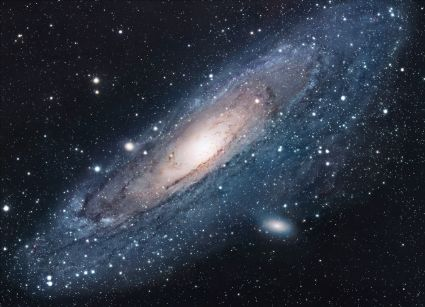
\includegraphics[scale=1.7]{universe}
\caption{The Universe}
\label{fig:universe}
\end{figure}



\section{Conclusion}
``I always thought something was fundamentally wrong with the universe'' \citep{adams1995hitchhiker}

\bibliographystyle{plain}
\bibliography{references}
\end{document}
